\documentclass[journal]{IEEEtran}


\ifCLASSINFOpdf
  \usepackage[pdftex]{graphicx}
\else
   \usepackage[dvips]{graphicx}
\fi

\usepackage{color}

\usepackage{url}
%\usepackage{showkeys}
\usepackage{siunitx}

% correct bad hyphenation here
\hyphenation{op-tical net-works semi-conduc-tor}

\definecolor{DarkGreen}{rgb}{0,0.45,0.08}
\usepackage{listings}
\lstset{language=C++,breaklines=true,breakatwhitespace=true,basicstyle=\small,prebreak = \raisebox{0ex}[0ex][0ex]{\ensuremath{\hookleftarrow}}, commentstyle=\color{DarkGreen}, tabsize=4}


\begin{document}
\title{CUDA raytracing algorithm for visualizing\\ discrete element model output}

\author{Anders Damsgaard Christensen,~\IEEEmembership{20062213}
\thanks{Contact: {anders.damsgaard@geo.au.dk}}%
\thanks{Webpage: {http://users-cs.au.dk/adc}}%
\thanks{Manuscript, last revision: \today.}}

% The paper headers
\markboth{Data Parallel Computing 2011}{Christensen: CUDA raytracing algorithm for visualizing DEM output}

% make the title area
\maketitle


\begin{abstract}
%\boldmath
A raytracing algorithm is constructed using the CUDA API for visualizing output from a CUDA discrete element model, which outputs spatial information in dynamic particle systems. 
The raytracing algorithm is optimized with constant memory and compilation flags, and performance is measured as a function of the number of particles and the number of pixels. The execution time is compared to equivalent CPU code, and the speedup under a variety of conditions is found to have a mean value of 55.6 times.
\end{abstract}
\begin{IEEEkeywords}
CUDA, discrete element method, raytracing
\end{IEEEkeywords}


\IEEEpeerreviewmaketitle


\section{Introduction}
\IEEEPARstart{V}{isualizing} systems containing many spheres using traditional object-order graphics rendering can often result in very high computational requirements, as the usual automated approach is to construct a meshed surface with a specified resolution for each sphere. The memory requirements are thus quite high, as each surface will consist of many vertices. Raytracing \cite{Whitted:1980} is a viable alternative, where spheric entities are saved as data structures with a centre coordinate and a radius. The rendering is performed on the base of these values, which results in a perfectly smooth surfaced sphere. To accelerate the rendering, the algorithm is constructed utilizing the CUDA API \cite{Nvidia-1:2010}, where the problem is divided into $n\times m$ threads, corresponding to the desired output image resolution. Each thread iterates through all particles and applies a simple shading model to determine the final RGB values of the pixel.

Previous studies of GPU or CUDA implementations of ray tracing algorithms reported major speedups, compared to corresponding CPU applications (e.g. \cite{Horn:2007,Shih:2009,Popov:2007,Luebke:2008}). None of the software was however found to be open-source and GPL licensed, so a simple raytracer was constructed, customized to render particles, where the data was stored in a specific data format.

\subsection{Discrete Element Method}
The input particle data to the raytracer is the output of a custom CUDA-based Discrete Element Method (DEM) application currently in development. The DEM model is used to numerically simulate the response of a drained, soft, granular sediment bed upon normal stresses and shearing velocities similar to subglacial environments under ice streams \cite{Evans:2006}. In contrast to laboratory experiments on granular material, the discrete element method \cite{Cundall:1979} approach allows close monitoring of the progressive deformation, where all involved physical parameters of the particles and spatial boundaries are readily available for continuous inspection. 

The discrete element method (DEM) is a subtype of molecular dynamics (MD), and discretizes time into sufficiently small timesteps, and treats the granular material as discrete grains, interacting through contact forces. Between time steps, the particles are allowed to overlap slightly, and the magnitude of the overlap and the kinematic states of the particles is used to compute normal- and shear components of the contact force. The particles are treated as spherical entities, which simplifies the contact search. The spatial simulation domain is divided using a homogeneous, uniform, cubic grid, which greatly reduces the amount of possible contacts that are checked during each timestep. The grid-particle list is sorted using Thrust\footnote{\url{http://code.google.com/p/thrust/}}, and updated each timestep. The new particle positions and kinematic values are updated by inserting the resulting force and torque into Newton's second law, and using a Taylor-based second order integration scheme to calculate new linear and rotational accelerations, velocities and positions.

\subsection{Application usage}
The CUDA DEM application is a command line executable, and writes updated particle information to custom binary files with a specific interval. This raytracing algorithm is constructed to also run from the command line, be non-interactive, and write output images in the PPM image format. This format is chosen to allow rendering to take place on cluster nodes with CUDA compatible devices.

Both the CUDA DEM and raytracing applications are open-source\footnote{\url{http://users-cs.au.dk/adc/files/sphere.tar.gz}}, although still under heavy development. 

This document consists of a short introduction to the basic mathematics behind the ray tracing algorithm, an explaination of the implementation using the CUDA API \cite{Nvidia-1:2010} and a presentation of the results. The CUDA device source code  and C++ host source code for the ray tracing algorithm can be found in the appendix, along with instructions for compilation and execution of the application.


\section{Ray tracing algorithm}
The goal of the ray tracing algorithm is to compute the shading of each pixel in the image \cite{Shirley:2009}. This is performed by creating a viewing ray from the eye into the scene, finding the closest intersection with a scene object, and computing the resulting color. The general structure of the program is demonstrated in the following pseudo-code:
\begin{lstlisting}[basicstyle=\footnotesize]
for each pixel do
  compute viewing ray origin and direction
  iterate through objects and find the closest hit
  set pixel color to value computed from hit point, light, n
\end{lstlisting}
The implemented code does not utilize recursive rays, since the modeled material grains are matte in appearance.

\subsection{Ray generation}
The rays are in vector form defined as:
\begin{equation}
  \mathbf{p}(t) = \mathbf{e} + t(\mathbf{s} - \mathbf{e})
  \label{eq:raygen}
\end{equation}
The perspective can be either \emph{orthograpic}, where all viewing rays have the same direction, but different starting points, or use \emph{perspective projection}, where the starting point is the same, but the direction is slightly different \cite{Shirley:2009}. For the purposes of this application, a perspective projection was chosen, as it results in the most natural looking image. The ray data structures were held flexible enough to allow an easy implementation of orthographic perspective, if this is desired at a later point.

The ray origin $\mathbf{e}$ is the position of the eye, and is constant. The direction is unique for each ray, and is computed using:
\begin{equation}
  \mathbf{s} - \mathbf{e} = -d \mathbf{w} + u \mathbf{u} + v \mathbf{v}
  \label{eq:raydirection}
\end{equation}
where $\{\mathbf{u},\mathbf{v},\mathbf{w}\}$ are the orthonormal bases of the camera coordinate system, and $d$ is the focal length \cite{Shirley:2009}. The camera coordinates of pixel ($i,j$) in the image plane, $u$ and $v$, are calculated by:
\[ u = l + (r-l)(i+0.5)/n \]
\[ v = b + (t-b)(j+0.5)/m \]
where $l$, $r$, $t$ and $b$ are the positions of the image borders (left, right, top and bottom) in camera space. The values $n$ and $m$ are the number of pixels in each dimension.


\subsection{Ray-sphere intersection}
Given a sphere with a center $\mathbf{c}$, and radius $R$, a equation can be constrained, where $\mathbf{p}$ are all points placed on the sphere surface:
\begin{equation}
  (\mathbf{p} - \mathbf{c}) \cdot (\mathbf{p} - \mathbf{c}) - R^2 = 0
  \label{eq:sphere}
\end{equation}
By substituting the points $\mathbf{p}$ with ray equation \ref{eq:raygen}, and rearranging the terms, a quadratic equation emerges:
\begin{equation}
  (\mathbf{d}\cdot\mathbf{d})t^2 + 2\mathbf{d}\cdot(\mathbf{e}-\mathbf{c})t
  + (\mathbf{e}-\mathbf{c})\cdot(\mathbf{e}-\mathbf{c}) - R^2 = 0
  \label{eq:quad}
\end{equation}
The number of ray steps $t$ is the only unknown, so the number of intersections is found by calculating the determinant:
\begin{equation}
  \Delta = (2(\mathbf{d}\cdot(\mathbf{e}-\mathbf{c})))^2 - 4(\mathbf{d}\cdot\mathbf{d}) ( (\mathbf{e}-\mathbf{c})\cdot(\mathbf{e}-\mathbf{c}) - R^2
  \label{eq:Delta}
\end{equation}
A negative value denotes no intersection between the sphere and the ray, a value of zero means that the ray touches the sphere at a single point (ignored in this implementation), and a positive value denotes that there are two intersections, one when the ray enters the sphere, and one when it exits. In the code, a conditional branch checks wether the determinant is positive. If this is the case, the distance to the intersection in ray ``steps'' is calculated using:
\begin{equation}
  t = \frac{-\mathbf{d}\cdot(\mathbf{e}-\mathbf{c}) \pm \sqrt{\eta} } { (\mathbf{d}\cdot\mathbf{d})}
  \label{eq:intersect}
\end{equation}
where
\[ \eta = (\mathbf{d}\cdot(\mathbf{e}-\mathbf{c}))^2 - (\mathbf{d}\cdot\mathbf{d})( (\mathbf{e}-\mathbf{c})\cdot(\mathbf{e}-\mathbf{c}) - R^2) \]
Only the smallest intersection ($t_\text{minus}$) is calculated, since this marks the point where the sphere enters the particle. If this value is smaller than previous intersection distances, the intersection point $\mathbf{p}$ and surface normal $\mathbf{n}$ at the intersection point is calculated:
\begin{equation}
  \mathbf{p} = \mathbf{e} + t_\text{minus} \mathbf{d}
  \label{eq:intersection}
\end{equation}
\begin{equation}
  \mathbf{n} = 2(\mathbf{p}-\mathbf{c})
  \label{eq:normal}
\end{equation}
The intersection distance in vector steps ($t_\text{minus}$) is saved in order to allow comparison of the distance with later intersections. 

\subsection{Pixel shading}
The pixel is shaded using \emph{Lambertian} shading \cite{Shirley:2009}, where the pixel color is proportional to the angle between the light vector ($\mathbf{l}$) and the surface normal. An ambient shading component is added to simulate global illumination, and prevent that the spheres are completely black:
\begin{equation}
  L = k_a I_a + k_d I_d \max(0,(\mathbf{n}\cdot\mathbf{l}))
  \label{eq:shading}
\end{equation}
where the $a$ and $d$ subscripts denote the ambient and diffusive (Lambertian) components of the ambient/diffusive coefficients ($k$) and light intensities ($I$). The pixel color $L$ is calculated once per color channel.


\subsection{Computational implementation}
The above routines were first implemented in CUDA for device execution, and afterwards ported to a CPU C++ equivalent, used for comparing performance. The CPU raytracing algorithm was optimized to shared-memory parallelism using OpenMP \cite{Chapman:2007}. The execution method can be chosen when launching the raytracer from the command line, see the appendix for details. In the CPU implementation, all data was stored in linear arrays of the right size, ensuring 100\% memory efficiency.


\section{CUDA implementation}
When constructing the algorithm for execution on the GPGPU device, the data-parallel nature of the problem (SIMD: single instruction, multiple data) is used to deconstruct the rendering task into a single thread per pixel. Each thread iterates through all particles, and ends up writing the resulting color to the image memory.

The application starts by reading the discrete element method data from a custom binary file. The particle data, consisting of position vectors in three-dimensional Euclidean space ($\mathbf{R}^3$) and particle radii, is stored together in a \texttt{float4} array, with the particle radius in the \texttt{w} position. This has large advantages to storing the data in separate \texttt{float3} and \texttt{float} arrays; Using \texttt{float4} (instead of \texttt{float3}) data allows coalesced memory access \cite{Nvidia-2:2010} to the arrays of data in device memory, resulting in efficient memory requests and transfers \cite{Nyland:2007}, and the data access pattern is coherent and convenient. Other three-component vectors were also stored as \texttt{float4} for the same reasons, even though this sometimes caused a slight memory redundancy. The image data is saved in a three-channel linear \texttt{unsigned char} array. Global memory access are coalesced whenever possible.
Divergent branches in the kernel code were avoided as much as possible \cite{Nvidia-2:2010}.

\begin{figure}[!t]
\centering
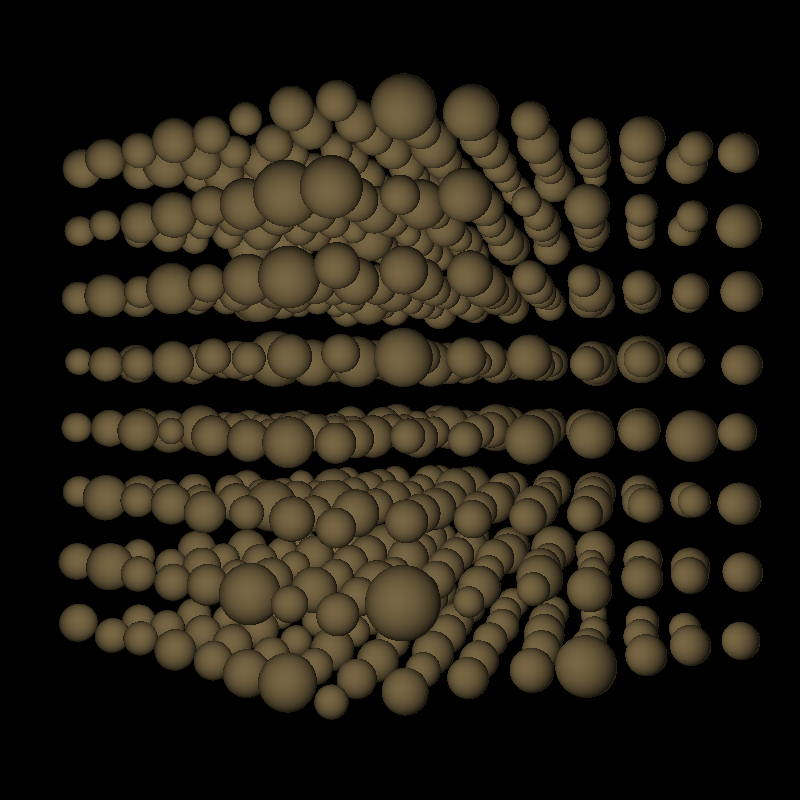
\includegraphics[width=0.47\textwidth]{np500.png}
\caption{Sample output of GPU raytracer rendering of \num{512} particles.}
\label{fig:np500.png}
\end{figure}


\begin{figure}[!t]
\centering
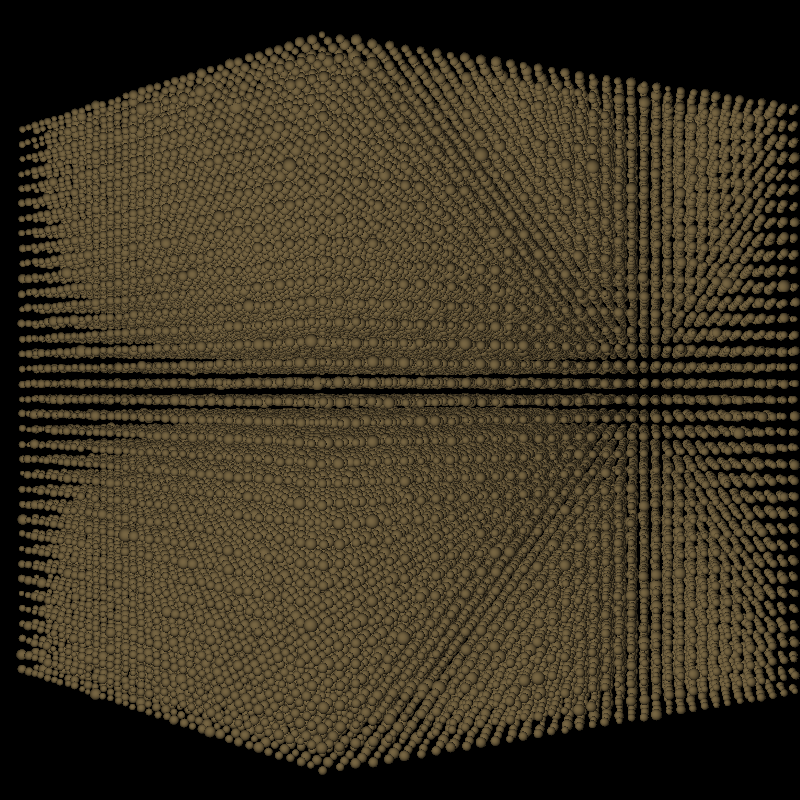
\includegraphics[width=0.47\textwidth]{np50000.png}
\caption{Sample output of GPU raytracer rendering of \num{50653} particles.}
\label{fig:np50000.png}
\end{figure}

The algorithm starts by allocating memory on the device for the particle data, the ray parameters, and the image RGB values. Afterwards, all particle data is transfered from the host- to the device memory.

All pixel values are initialized to $[R,G,B] = [0,0,0]$, which serves as the image background color. Afterwards, a kernel is executed with a thread for each pixel, testing for intersections between the pixel's viewing ray and all particles, and returning the closest particle. This information is used when computing the shading of the pixel. 

After all pixel values have been computed, the image data is transfered back to the host memory, and written to the disk. The application ends by liberating dynamically allocated memory on both the device and the host.

\subsection{Thread and block layout}
The thread/block layout passed during kernel launches is arranged in the following manner:
\begin{lstlisting}
  dim3 threads(16, 16);
  dim3 blocks((width+15)/16, (height+15)/16);
\end{lstlisting}
The image pixel position of the thread can be determined from the thread- and block index and dimensions. The layout corresponds to a thread tile size of 256, and a dynamic number of blocks, ensured to fit the image dimensions with only small eventual redundancy \cite{Sanders:2010}. Since this method will initialize extra threads in most situations, all kernels (with return type \texttt{void}) start by checking wether the thread-/block index actually falls inside of the image dimensions:
\begin{lstlisting}
  int i = threadIdx.x + blockIdx.x * blockDim.x;
  int j = threadIdx.y + blockIdx.y * blockDim.y;
  unsigned int mempos = x + y * blockDim.x * gridDim.x;
  if (mempos > pixels)
    return;
\end{lstlisting}
The linear memory position (\texttt{mempos}) is used as the index when reading or writing to the linear arrays residing in global device memory.

\subsection{Image output}
After completing all pixel shading computations on the device, the image data is transfered back to the host memory, and together with a header written to a PPM\footnote{\url{http://paulbourke.net/dataformats/ppm/}} image file. This file is converted to the PNG format using ImageMagick.

\subsection{Performance}
Since this simple raytracing algorithm generates a single non-recursive ray for each pixel, which in turn checks all spheres for intersection, the application is expected to scale in the form of $O(n\times m \times N)$, where $n$ and $m$ are the output image dimensions in pixels, and $N$ is the number of particles.

The data transfer between the host and device is kept at a bare minimum, as the intercommunication is considered a bottleneck in relation to the potential device performance \cite{Nvidia-2:2010}. Thread synchronization points are only inserted were necessary, and the code is optimized by the compilers to the target architecture (see appendix). 

The host execution time was profiled using a \texttt{clock()} based CPU timer from \texttt{time.h}, which was normalized using the constant \texttt{CLOCKS\_PER\_SEC}. 

The device execution time was profiled using two \texttt{cudaEvent\_t} timers, one measuring the time spent in the entire device code section, including device memory allocation, data transfer to- and from the host, execution of the kernels, and memory deallocation. The other timer only measured time spent in the kernels. The threads were synchronized before stopping the timers. A simple CPU timer using \texttt{clock()} will \emph{not} work, since control is returned to the host thread before the device code has completed all tasks.

Figures \ref{fig:np-performance.pdf} and \ref{fig:px-performance.pdf} show the profiling results, where the number of particles and the image dimensions were varied. With exception of executions with small image dimensions, the kernel execution time results agree with the $O(n \times m \times N)$ scaling predicion.

\begin{figure}[!t]
\centering
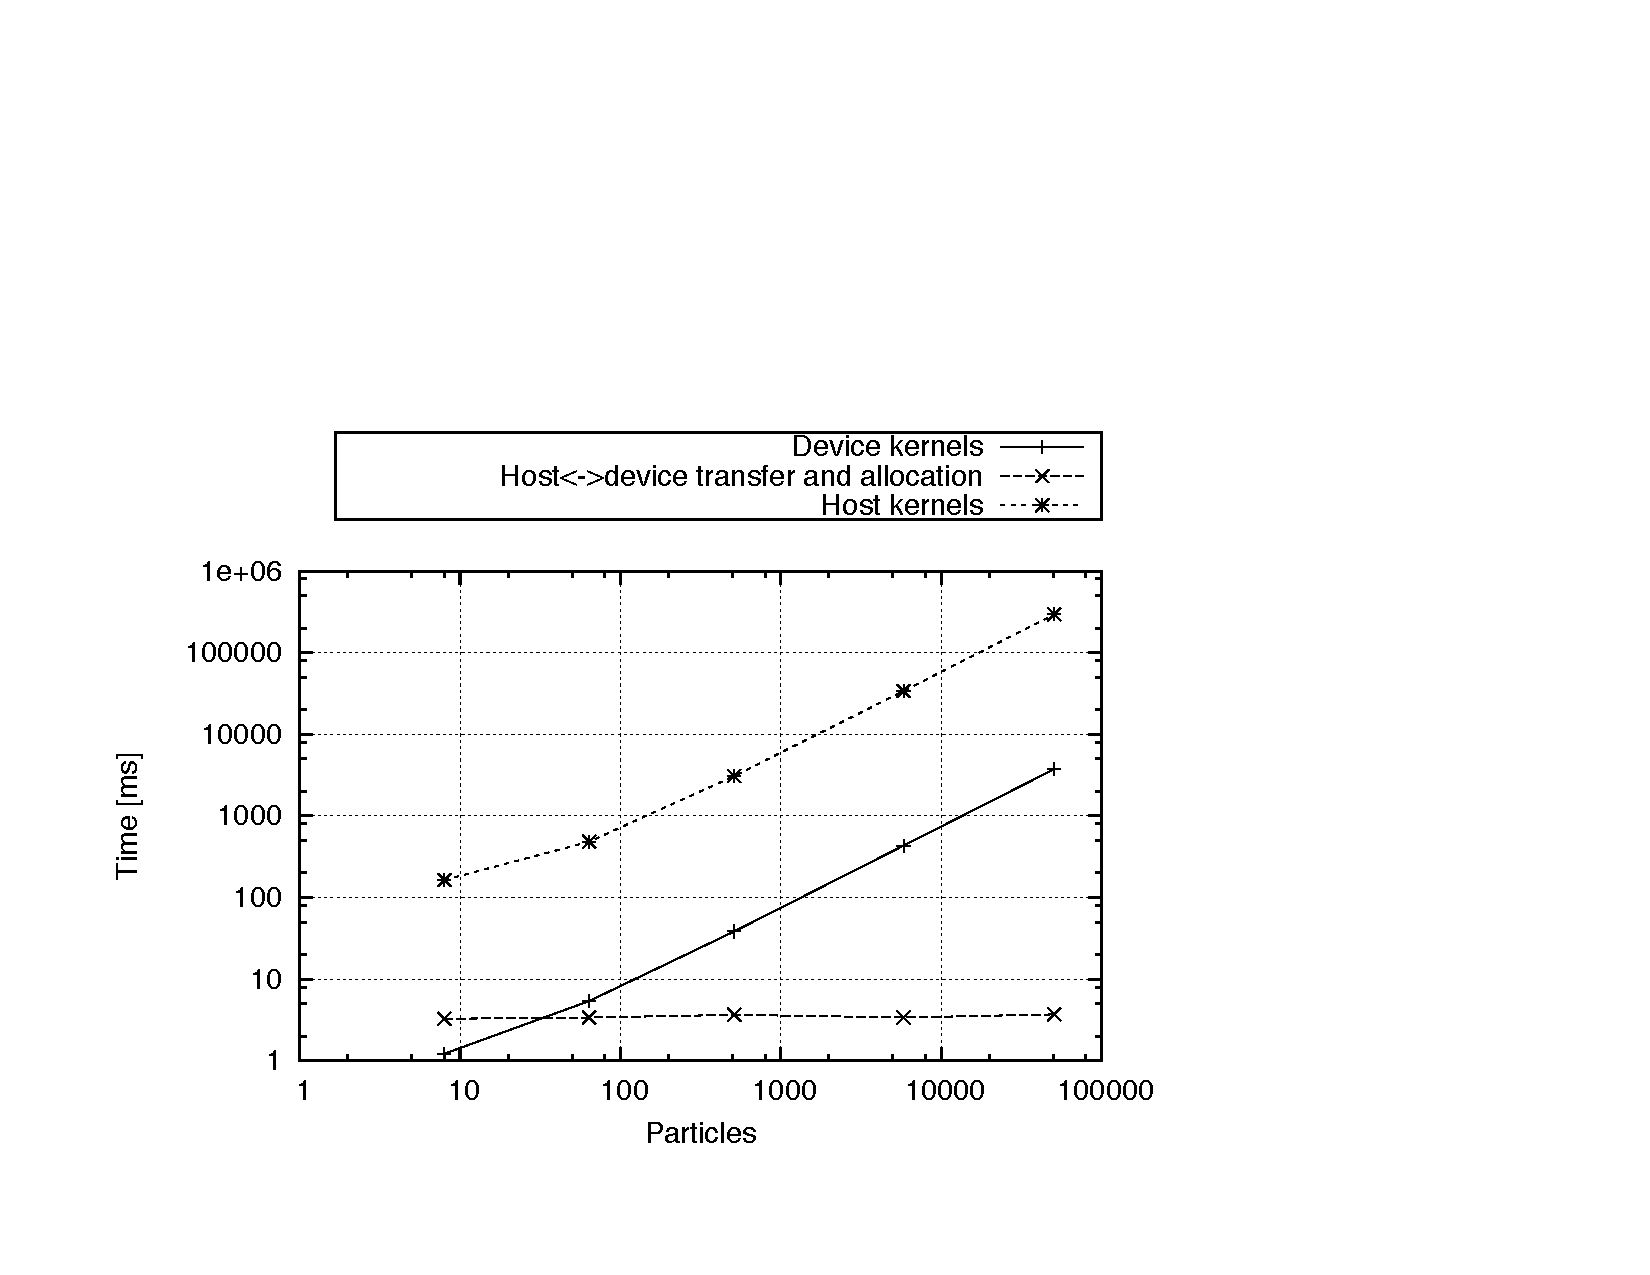
\includegraphics[width=0.47\textwidth]{np-performance.pdf}
\caption{Performance scaling with varying particle numbers at image dimensions 800 by 800 pixels.}
\label{fig:np-performance.pdf}
\end{figure}

\begin{figure}[!t]
\centering
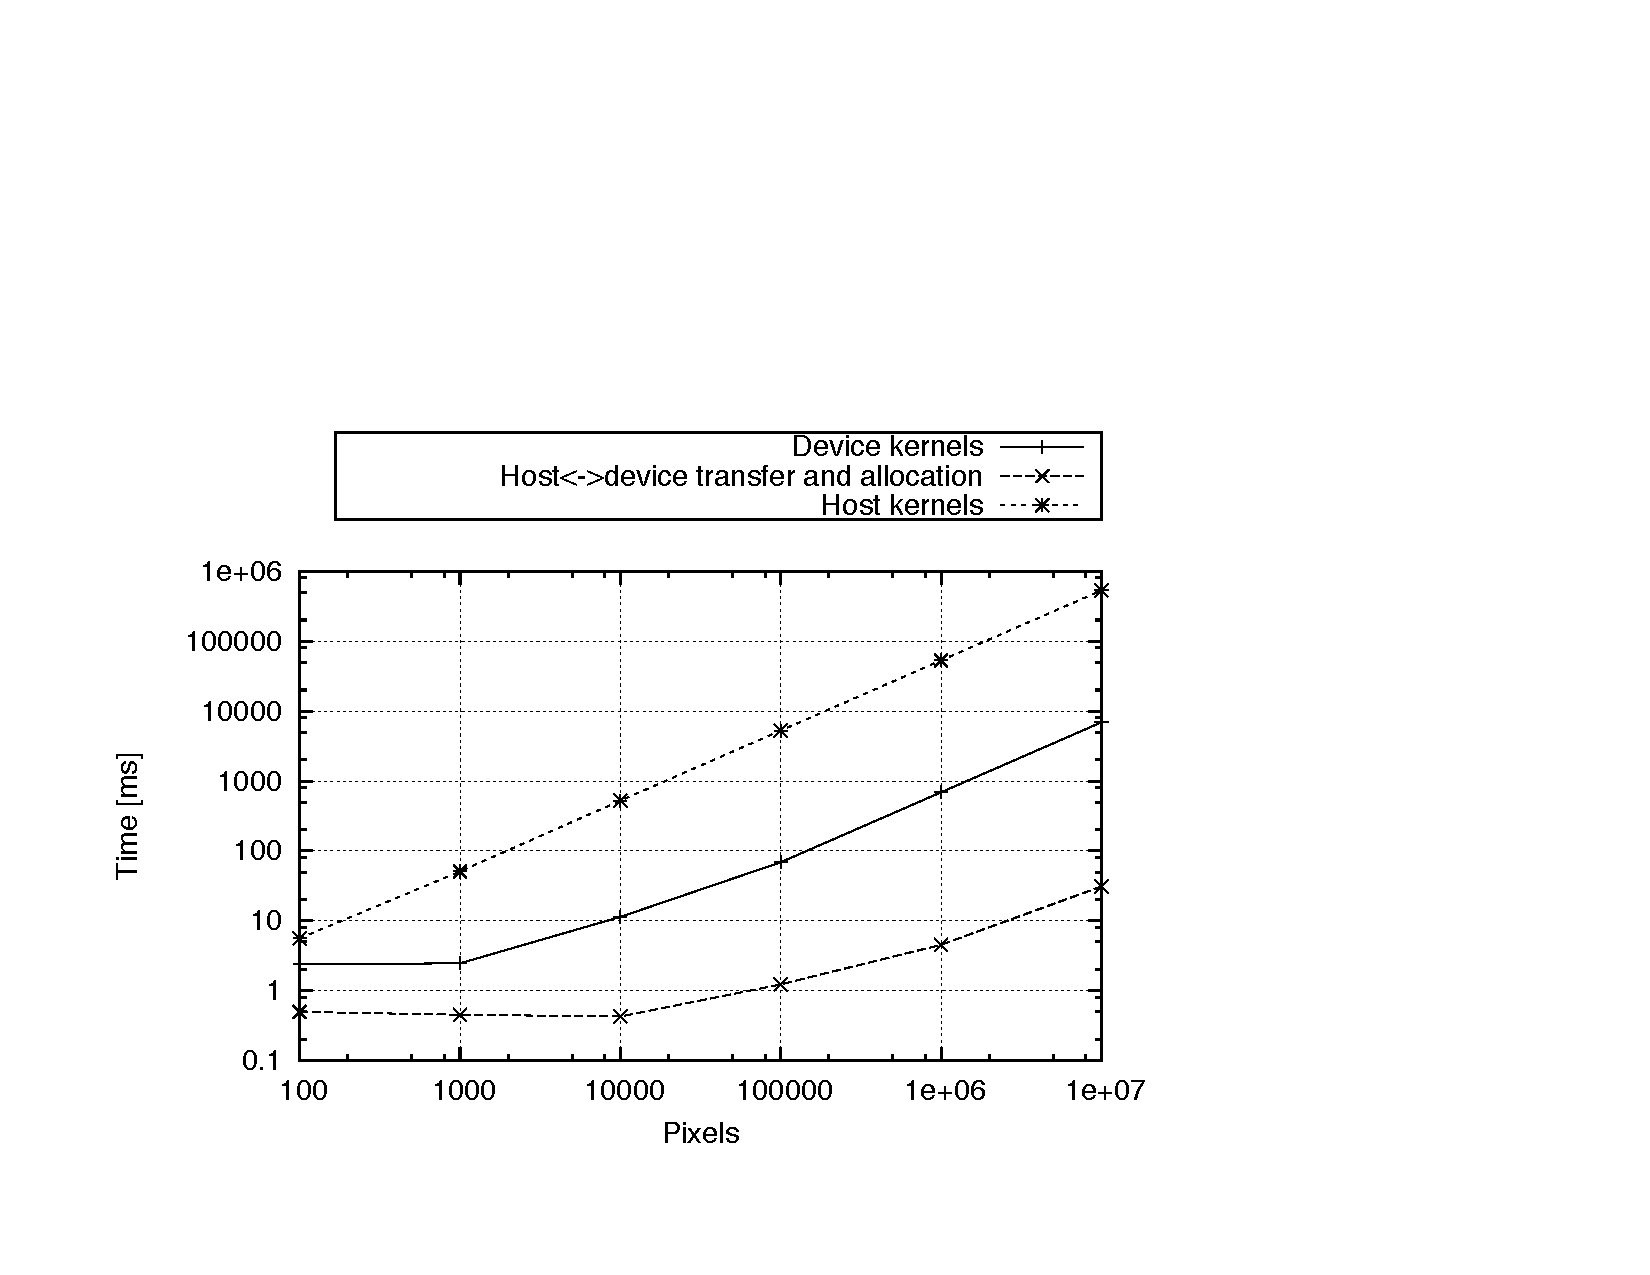
\includegraphics[width=0.47\textwidth]{px-performance.pdf}
\caption{Performance scaling with varying image dimensions ($n \times m$) with 5832 particles.}
\label{fig:px-performance.pdf}
\end{figure}

The device memory allocation and data transfer was also profiled, and turns out to be only weakly dependant on the particle numbers (fig. \ref{fig:np-performance.pdf}), but more strongly correlated to image dimensions (fig. \ref{fig:px-performance.pdf}). As with kernel execution times, the execution time converges against an overhead value at small image dimensions.

The CPU time spent in the host kernels proves to be linear with the particle numbers, and linear with the image dimensions. This is due to the non-existant overhead caused by initialization of the device code, and reduced memory transfer.

The ratio between CPU computational times and the sum of the device kernel execution time and the host---device memory transfer and additional memory allocation was calculated, and had a mean value of \num{55.6} and a variance of \num{739} out of the 11 comparative measurements presented in the figures. It should be noted, that the smallest speedups were recorded when using very small image dimensions, probably unrealistic in real use.

As the number of particles are not known by compilation, it is not possible to store particle positions and -radii in constant memory. Shared memory was also on purpose avoided, since the memory per thread block (64 kb) would not be sufficient in rendering of simulations containing containing more than \num{16000} particles (\num{16000} \texttt{float4} values). The constant memory was however utilized for storing the camera related parameters; the orthonormal base vectors, the observer position, the image dimensions, the focal length, and the light vector.

Previous GPU implementations often rely on k-D trees, constructed as an sorting method for static scene objects \cite{Horn:2007,Popov:2007}. A k-D tree implementation would drastically reduce the global memory access induced by each thread, so it is therefore the next logical step with regards to optimizing the ray tracing algorithm presented here.

\section{Conclusion}
This document presented the implementation of a basic ray tracing algorithm, utilizing the highly data-parallel nature of the problem when porting the work load to CUDA.
Performance tests showed the expected, linear correlation between image dimensions, particle numbers and execution time. Comparisons with an equivalent CPU algorithm showed large speedups, typically up to two orders of magnitude. This speedup did not come at a cost of less correct results.

The final product will come into good use during further development and completion of the CUDA DEM particle model, and is ideal since it can be used for offline rendering on dedicated, heterogeneous GPU-CPU computing nodes. The included device code will be the prefered method of execution, whenever the host system allows it.

\bibliographystyle{IEEEtran}
\bibliography{IEEEabrv,/Users/adc/Documents/University/BIB}



\appendices

\section{Test environment}
The raytracing algorithm was developed, tested and profiled on a mid 2010 Mac Pro with a \num{2.8} Ghz Quad-Core Intel Xeon CPU and a NVIDIA Quadro 4000 for Mac, dedicated to CUDA applications. The CUDA driver was version 4.0.50, the CUDA compilation tools release 4.0, V0.2.1221. The GCC tools were version 4.2.1. Each CPU core is multithreaded by two threads for a total of 8 threads.

The CUDA source code was compiled with \texttt{nvcc}, and linked to \texttt{g++} compiled C++ source code with \texttt{g++}. For all benchmark tests, the code was compiled with the following commands:
\begin{lstlisting}
g++ -c -Wall -O3 -arch x86_64 -fopenmp ... 
nvcc -c -use_fast_math -gencode arch=compute_20,code=sm_20 -m64 ...
g++ -arch x86_64 -lcuda -lcudart -fopenmp *.o -o rt
\end{lstlisting}
When profiling device code performance, the application was executed two times, and the time of the second run was noted. This was performed to avoid latency caused by device driver initialization.

The host system was measured to have a memory bandwidth of 4642.1 MB/s when transfering data from the host to the device, and 3805.6 MB/s when transfering data from the device to the host.

\ifCLASSOPTIONcaptionsoff
  \newpage
\fi


\section{Source code}
The entire source code, as well as input data files, can be found in the following archive
\url{http://users-cs.au.dk/adc/files/sphere-rt.tar.gz}
The source code is built and run with the commands:
\begin{lstlisting}
  make
  make run
\end{lstlisting}
With the \texttt{make run} command, the Makefile uses ImageMagick to convert the PPM file to PNG format, and the OS X command \texttt{open} to display the image. Other input data files are included with other particle number magnitudes. The syntax for the raytracer application is the following:
\begin{lstlisting}
  ./rt <CPU | GPU> <sphere-binary.bin> <width> <height> <output-image.ppm>
\end{lstlisting}
This appendix contains the following source code files:
\lstlistoflistings

\subsection{CUDA raytracing source code}
%\subsubsection{rt\_kernel.h}
\lstinputlisting[caption={rt-kernel.h},label={rt-kernel.h},numbers=left,breaklines=true,xleftmargin=15pt,basicstyle=\scriptsize]{../rt-kernel.h}

%\subsubsection{rt\_kernel.cu}
\lstinputlisting[caption={rt-kernel.cu},label={rt-kernel.cu},numbers=left,breaklines=true,xleftmargin=15pt,basicstyle=\scriptsize]{../rt-kernel.cu}

\subsection{CPU raytracing source code}
%\subsubsection{rt\_kernel\_cpu.h}
\lstinputlisting[caption={rt-kernel-cpu.h},label={rt-kernel-cpu.h},numbers=left,breaklines=true,xleftmargin=15pt,basicstyle=\scriptsize]{../rt-kernel-cpu.h}

%\subsubsection{rt\_kernel\_cpu.cpp}
\lstinputlisting[caption={rt-kernel-cpu.cpp},label={rt-kernel-cpu.cpp},numbers=left,breaklines=true,xleftmargin=15pt,basicstyle=\scriptsize]{../rt-kernel-cpu.cpp}



\clearpage









% You can push biographies down or up by placing
% a \vfill before or after them. The appropriate
% use of \vfill depends on what kind of text is
% on the last page and whether or not the columns
% are being equalized.

%\vfill

% Can be used to pull up biographies so that the bottom of the last one
% is flush with the other column.
%\enlargethispage{-5in}



% that's all folks
\end{document}


